\documentclass{article}

% Language setting
% Replace `english' with e.g. `spanish' to change the document language
\usepackage[french]{babel}
\usepackage[fleqn]{amsmath} % Aligner les équations à gauche


% Set page size and margins
% Replace `letterpaper' with`a4paper' for UK/EU standard size
\usepackage[letterpaper,top=2cm,bottom=2cm,left=3cm,right=3cm,marginparwidth=1.75cm]{geometry}

% Useful packages

\usepackage{amsmath}
\usepackage{graphicx}
\usepackage{subcaption}
\usepackage[colorlinks=true, allcolors=blue]{hyperref}

\title{TD 10 - Ondes électromagnétiques dans le vide}
\author{IPESUP - PC }
\date{27/11/24}

\begin{document}
\maketitle

\section{Rappels de cours}

Les champs $\vec{B}$ et $\vec{E}$ vérifient l'équation d'Euler tridimensionnelle : \\

$\Delta \vec{B}(M, t) = \frac{1}{c^2} \frac{\partial^2 \vec{B}(M, t)}{\partial t^2}$, avec $c=\frac{1}{\sqrt{\epsilon_0 \mu_0}}$ \\

\textbf{Définition}: Une onde plane est une onde dont les surfaces d'onde sont des plans. Pour rappel, on définit une surface d'onde comme l'ensemble des points $M$ tels que $\vec{E}(M, t) = \vec{E}_0$  \\

\textbf{Quelques concepts: }
\begin{enumerate}
  \item Relation de dispersion: relation entre $\omega$ et le vecteur d'onde. 
  \item Vitesse de phase $v_\phi = \frac{\omega}{k}$
  \item Vitesse de groupe $v_g = \frac{d\omega}{dk}$
  \item Bilan énergétique : $div(\Pi) + \frac{\partial u_{em}}{\partial t } = -\vec{j} \cdot \vec{E}$     \\[1cm]
\end{enumerate}

\textbf{Propriétés des OPPH}: \\
\begin{enumerate}
  \item Les champs $\vec{E}$ et $\vec{B}$ sont orthogonaux entre eux et à la direction de propagation.
  \item Les champs $\vec{E}$ et $\vec{B}$ sont en phase.
  \item $\vec{B} = \frac{\vec{k}}{\omega} \wedge \vec{E}$
  \item Relation de dispersion: $\omega^2 = c^2 k^2$\\[0.5cm]
\end{enumerate}

\textbf{Capacités exigibles}: \\
\begin{enumerate}
  \item Relation entre $\vec{E}$ et $\vec{B}$ pour une OPPH. 
  \item Retrouver la relation de dispersion pour une OPPH. 
  \item Calculer la vitesse de phase et de groupe pour une OPPH.
\end{enumerate}



\section{Onde électromagnétique dans le vide}

On considère une onde électromagnétique se propageant dans le vide. On la représentation complexe du champ électrique de cette onde : \\



\[
\vec{E} = \left\{
\begin{array}{l}
0 \\
E_0 cos(\frac{\pi y }{a}) exp(i(\omega t - k_0 z)) \\
\underline{\alpha} E_0 sin (\frac{\pi y}{a}) exp(i(\omega t - k_0 z)) \\
\end{array}
\right.
\]

avec $\underline{\alpha}$ un nombre complexe et $k_0$ positif. 

\begin{enumerate}
  \item Déterminer $\underline{\alpha}$ et $k_0$ en fonction de $E_0$, $\omega$, $a$ et $c$. 
  \item Déterminer le champ magnétique $\vec{B}$ associé à cette onde. 
  \item Calculer le vecteur de Poynting et sa valeur moyenne dans le temps. 
  \item Calculer la valeur moyenne dans le temps de la densité volumique d'énergie. 
\end{enumerate}

\section{Guide d'ondes rectangulaire}
Quatre plans métalliques parfaitement conducteurs (sur la figure ci-dessous x=0, x=a, y=0,
y=b) délimitent un guide d’onde de longueur infinie suivant Oz, de section droite rectangulaire et dans lequel règne le vide (permitivité $\epsilon_0$, perméabilité $\mu_0$).
On se propose d’étudier la propagation dans ce guide suivant la direction Oz d’une onde
électromagnétique monochromatique de pulsation $\omega$, dont le champ électrique s’écrit :
$\vec{E}=f(x,y)cos(\omega t-k_g z)\vec{u_x}$. Dans cette expression : f désigne une fonction réelle des 
variables y et x, et $ k_g$ est une constante positive. On posera $k_g=\frac{2\pi}{\lambda_g}$, où $\lambda_g$ est  la  "longueur d’onde
guidée" et on notera : $k_0 = \frac{2\pi}{\lambda_0}=\frac{\omega}{c}$


\begin{enumerate}
    \item Montrer que $f$ ne dépend que de y puis déterminer l'équation différentielle à laquelle est soumise $f(y)$.
    \item Résoudre cette équation et introduire un entier $n$ correspondant à différents modes propres. 
    \item Déterminer $\vec{B}$.
    \item Exprimer $k_g$ en fonction de $\omega$, c, n et b. En déduire $\lambda_g$ en fonction de $\lambda_0$, b et n.
    \item Montrer qu’il existe une fréquence de coupure $f_c$ en dessous de laquelle il n’y a plus propagation.
    \item Exprimer la vitesse de phase $v_\phi$ de l’onde en fonction de c, n et du rapport $\frac{f}{f_c}$, $f$ étant la fréquence de l'onde.
    \item  Donner l’expression du vecteur de Poynting $\vec{\Pi}$ . Quelle est
    la valeur moyenne  $<\vec{\Pi}>$ dans le temps de ce vecteur ?
    En déduire la puissance moyenne transmise par une section droite du guide d’ondes.
    \item Calculer la valeur moyenne, dans le temps de la densité d’énergie volumique de l’énergie
    électromagnétique $<u>$
    \item A l’aide des résultats précédents, déduire la vitesse de propagation $v_e$ de l’énergie.
    Quelle relation simple peut-on constater entre $v_e $ et $v_\phi$ ? \\[2cm]
\end{enumerate}


\begin{figure}[h]
  \centering
  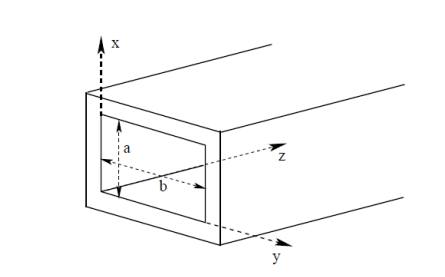
\includegraphics[width=0.4\textwidth]{schéma_guide_d'ondes.png}
  \label{fig:schéma_guide_'ondes}
\end{figure}


\section{Pression de radiation}

\begin{enumerate}
    \item Soit une onde plane, monochromatique, de fréquence $\nu$ se propageant le long des x croissants, dont le champ électrique est $\vec{E}(x,t)=E_0cos(\omega t-kx)\vec{u_y}$. Soit  $\mathcal{E}$ l'éclairement (défini par la puissance moyenne qui traverse une surface d'aire unité perpendiculaire à la direction de propagation). Exprimer $\mathcal{E}$ en fonction de $\epsilon_0, c $ et $E_0$. 
    \item On considère cette onde comme un faisceau de photons se propageant le long des x croissants. 
    \begin{enumerate}
        \item Exprimer $N_0$ le nombre de photons traversant par unité de temps l'unité de surface perpendiculaire à $Ox$ en fonction de $\mathcal{E}$ et de $\nu$. 
        \item L'onde arrive sur une surface plane perpendiculaire à $Ox$, d'aire S, et parfaitement réfléchissante. On étudie le rebondissement des photons sur cette surface. 
        \\
        Quelle est la quantité de mouvement reçue par la paroi au cours d'un choc photon-paroi ? \\
        Quelle est la force subie par la paroi en fonction de $\mathcal{E}$, $S$ et $c$ ? 
        Exprimer la pression $p$ subie par la paroi en fonction de $\mathcal{E}$ et $c$ puis en fonction de $\epsilon_0$ et $E_0$. 
        \item Reprendre la question ci-dessus lorsque la paroi est parfaitement aborbante. 
        \item Calculer $\mathcal{E}$, $E_0$ et $p$ sur une paroi totalement absorbante pour un laser ayant un diamètre $d$=5,00 mm et une puissance moyenne $\mathcal{P}$=100 W (laser utilisé industriellement pour la découpe de feuilles). 
    \end{enumerate}
    \item 
    \begin{enumerate} 
    \item L'onde est maintenant absorbée par une sphère de rayon $a$, bien inférieur au rayon du faisceau. Quelle est, en fonction de $\mathcal{E}$, $E_0$ et $p$, la force $\vec{F}$ subie par la sphère ? 
    \item Le soleil donne au voisinage de la Terre l'éclairement $\mathcal{E}$ = 1,4 $\times 10^3 W.m^{-2}$. L'émission est isotrope. Sur une surface de dimensions petites devant D, l'onde arrivant du Soleil est quasi plane. \\
    Quelle est la puissance $\mathcal{P_0}$ émise par le Soleil ? \\
    Un objet sphérique de rayon $a$, de masse volumique $\mu$ est situé à une distance $r$ du Soleil et absorbe totalement le rayonnement solaire. Evaluer le rapport entre la force due à l'absorbtion du rayonnement solaire et a force gravitationelle exercée par le Soleil sur cet objet dans les deux cas suivants:\\
    - Cas d'une météorite : $\mu = 3,0\times10^3 kg.m^{-3}$ et $a=1,0m$\\
    - Cas d'une poussière interstellaire: $\mu=1,0\times10^3kg.m^{-3}$
    \\ Commenter.
    \item Quelle est la surface minimale de la voile solaire d'un vaisseau spatial pour que celui-ci quitte l'attraction solaire ?  \\[2cm]
    \end{enumerate}
\end{enumerate}

\begin{figure}[h]
  \centering
  
\includegraphics[width=0.4\textwidth]{meme.jpg}
  % \label{fig:schéma_guide_'ondes}
\end{figure}

\end{document}

